\documentclass[letterpaper,12pt]{report}

\usepackage{multirow,titlesec}
\usepackage{graphicx,url,tabularx,color,xcolor}

\usepackage{ucs}
\usepackage[utf8x]{inputenc}
\usepackage[spanish]{babel}

\usepackage{fancyhdr}
\usepackage{lastpage}


\usepackage[top=2.5cm, bottom=2.5cm, left=2cm, right=2cm]{geometry}

\pagestyle{fancy}

\usepackage{setspace}
\onehalfspacing

\renewcommand{\thesection}{\arabic{section}}

\addto\captionsspanish{\renewcommand{\contentsname}{Índice}}

\definecolor{azultitulo}{HTML}{004A4F}

\makeatletter
\def\headrule{{\color{azultitulo}\if@fancyplain\let\headrulewidth\plainheadrulewidth\fi
\hrule\@height\headrulewidth\@width\headwidth
\vskip-\headrulewidth}}
\makeatother

\titleformat{\section}
{\color{azultitulo}\normalfont\Large\bfseries}
{\color{azultitulo}\thesection}{1em}{}

\begin{document}

\begin{titlepage}
\fontsize{18pt}{20pt}\selectfont
\ \\[1.5cm]
\hangindent=3cm
\textbf{Curriculum Vitae} \newline \newline
\fontsize{28pt}{28pt}\selectfont
\color{azultitulo}\textbf{José R. Carrero L.}\color{black}
\vfill

\fontsize{12pt}{12pt}\selectfont
\begin{center}
\begin{tabularx}{.8\textwidth}{|>{\centering}X|>{\centering}X|>{\centering}X|>{\centering\arraybackslash}X|}
\hline
\textbf{Fecha} & \textbf{Detalle} & \textbf{Ejecutó} & \textbf{Aprobó} \\
\hline
02/11/2012 & Revisión 1 & Carrero, J. & \\
\hline
13/01/2012 & Versión Original & Carrero, J. & \\
\hline
\hline
\end{tabularx}
\end{center}

\thispagestyle{fancy}
\fancyhead{}
\renewcommand{\headrulewidth}{0pt}
\renewcommand{\footrulewidth}{0.5pt}
\fancyfoot{}
\fancyfoot[CO,CE]{josercl@gmail.com}

\end{titlepage}

\setcounter{page}{2}
\tableofcontents
\thispagestyle{fancy}
\renewcommand{\headrulewidth}{0pt}
\renewcommand{\footrulewidth}{0.5pt}
\clearpage

\pagestyle{fancy}
\fancyhead{}
\renewcommand{\headrulewidth}{1.2pt}
\fancyhead[RO,RE]{\color{azultitulo}\textbf{José R. Carrero L.}}
\renewcommand{\footrulewidth}{0.5pt}
\fancyfoot{}
\fancyfoot[RO,RE]{\textbf{Página \thepage\ de \pageref{LastPage}}}

\section{Datos Personales}

    \begin{tabular}{r p{2.4in} p{46mm}}
    \textbf{Nombre} & José Rafael Carrero León & \multirow{8}{*}{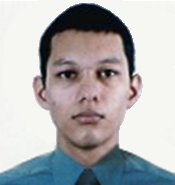
\includegraphics[scale=.5]{foto_curriculum}}\\
    \textbf{Fecha de Nacimiento} & 17-09-1982 & \\
    \textbf{Edad} & 30 años & \\
    \textbf{Nacionalidad} & Venezolana & \\
    \textbf{Estado Civil} & Soltero & \\
    \textbf{Domicilio} & Urb. Río Aro, Villas Sta. Elena\newline Mz. 15, No k-05 \newline Puerto Ordaz, Edo. Bolívar, Venezuela & \\
    \textbf{Teléfono Hab.:} & +58 0286-9520837 & \\
    \textbf{Teléfono Móvil:} & +58 0416-3105412 & \\
    \end{tabular}

\section{Formación Universitaria}
    
    Título: Ingeniero en Computación. Otorgado por: Universidad Simón Bolívar. Marzo 2006

\section{Antecedentes Profesionales}

    \begin{itemize}

        \item{ESEPRIN C.A. (Puerto Ordaz, Edo. Bolívar)}
        \begin{itemize}
        \item{\textbf{Período}: Febrero 2011 - Presente}
        \item{\textbf{Actividades Desarrolladas:}}
            \begin{enumerate}
            \item Desarrollo e implementación del Sistema de Ejecución de Manufactura (MES)
                \begin{itemize}
                \item Sistema desarrollado en PHP, haciendo uso del patrón MVC
                \item Diseño de base de datos en PostgreSQL
                \item Implementación de un cliente OPC en Python para obtener información en tiempo real
                \item Diseño e implementación de programa de análisis del estado de la línea de producción basado en reglas lógicas y valores de variables en tiempo real
                \end{itemize}
            \item Instalación y Configuración de Servicios
                \begin{itemize}
                \item Instalación de sistema operativo de la máquina de desarrollo (Debian Squeeze) y pruebas (Archlinux)
                \item Instalación de entorno de desarrollo Linux/Apache/Postgresql/PHP
                \item Instalación de servidor de control de versiones de Planos (Subversion)
                \item Instalación de servidor de control de versiones de código fuente (Git)
                \end{itemize}
            \end{enumerate}
        \end{itemize}
    
        \item{Desarrollador \emph{Freelance}}
        \begin{itemize}
        \item{\textbf{Período}: Octubre 2010 - Febrero 2011}
        \item{\textbf{Actividades Desarrolladas:}}
            \begin{enumerate}
            \item Migración del Sistema para Recursos Humanos de la Dirección Ejecutiva de la Magis\-tratura - Octubre 2010
	            \begin{itemize}
	            \item Migración de la tecnología usada en el sistema de Active Server Pages (ASP) a Java
	            \item La nueva versión fue desarrollada en Java 1.6 bajo la plataforma Struts 2
	            \item Base de datos implementada en Oracle 10g
	            \end{itemize}
            \item Desarrollo e Implementación del sitio web \url{http://www.musicasacra.com.ve} - Octubre 2010
	            \begin{itemize}
		            \item Sitio desarrollado en PHP y MySQL, usando el ambiente de trabajo MVC Codeigniter
		            \item Los aspectos de interfaz fueron desarrollados en CSS, HTML y jQuery
	            \end{itemize}
            \end{enumerate}
        \end{itemize}

        \item{Consorcio Kairos IT (Puerto Ordaz, Edo. Bolívar)}
        \begin{itemize}
        \item{\textbf{Período:} Julio 2009 - Diciembre 2011}
        \item{\textbf{Puesto y Tareas:} Analista Integral III}
        \item{\textbf{Actividades Desarrolladas:}}
            \begin{enumerate}
                \setcounter{enumi}{2}
                \item Parte del equipo de desarrolladores del sistema de nómina del Grupo Principal
                \begin{itemize}
                    \item Sistema desarrollado usando PHP, MSSQL Server y un ambiente de trabajo MVC desarrollado en la empresa
                    \item Implementación de consultas para la generación de reportes de gestión de nómina/personal
                \end{itemize}
                \item Parte del grupo de trabajo encargado de desarollar el Sistema de Notificaciones Legales www.notifica.net
                  \begin{itemize}
                    \item Sistema desarrollado usando PHP, MySQL, y el Ambiente de Trabajo MVC CodeIgniter
                    \item Los aspectos del cliente fueron elaborados usando CSS, HTML y Javascript usando la librería jQuery.
                    \item Implementación de la firma de correos electrónicos y documentos PDF usando openssl y Java
                    \item Dise\~{n}o e implementación de la base de datos del sistema
                  \end{itemize}
                \item Encargado del desarrollo y mantenimiento del sitio web de la empresa http://www.kairosit.net.
                \item Instalacion del servidor de desarrollo
                    \begin{itemize}
                        \item Instalación del entorno LAMP (Linux, Apache, MySQL, PHP)
                        \item Configuración del firewall (iptables)
                        \item Instalación y configuración del control de versiones (SVN)
                    \end{itemize}
            \end{enumerate}
        \end{itemize}


        \item{IST Consultores (Puerto Ordaz, Edo. Bolívar)}
        \begin{itemize}
            \item{\textbf{Período:} Junio 2008 - Julio 2009}
            \item{\textbf{Puesto y Tareas:} Analista Integral II}
            \item{\textbf{Actividades Desarrolladas:}}
            \begin{enumerate}
                \setcounter{enumi}{6}
                \item Parte del grupo de trabajo de desarrollo de la intranet del Banco Central de Venezuela
            	    \begin{itemize}
	                    \item Optimizacion de consultas a la base de datos dentro del sistema
	                    \item Dise\~{n}o y puesta en práctica de las pruebas de stress del servidor de la intranet del BCV
	                \end{itemize}
            \end{enumerate}
        \end{itemize}    

        \item{Universidad Simón Bolívar - Decanato de Investigación y Desarrollo}
        \begin{itemize}
            \item{\textbf{Período:} Enero 2007 - Diciembre 2007}
            \item{\textbf{Puesto y Tareas:} Jefe de la Unidad de Informática}
            \item{\textbf{Actividades Desarrolladas:}}
            \begin{itemize}
                \item Webmaster de la unidad
                \item Administrador del servidor de base de datos del decanato
                \item Parte del grupo de desarrolladores de sistemas
                \begin{itemize}
            	    \item Desarrollo del Sistema de Solicitudes de Financiamiento para trabajos de investigación.
                \end{itemize}
            \end{itemize}
        \end{itemize}

        \item{Universidad Simón Bolívar - Decanato de Postgrado}
        \begin{itemize}
            \item{\textbf{Período:} Enero 2007 - Diciembre 2007}
            \item{\textbf{Puesto y Tareas:} Encargado Unidad de Informática}
            \item{\textbf{Actividades Desarrolladas:}}
            \begin{itemize}
                \item Webmaster de la unidad
                \item Administrador del servidor de base de datos del decanato
                \item Desarrollador de sistemas en PHP y Java (JSP, Tomcat)
            \end{itemize}
        \end{itemize}

    \end{itemize}


\section{Conocimientos Específicos}

    \begin{itemize}
    \item
    \textbf{Dominio de Lenguajes de Especificación y Programación:} BASIC, C, Ensamblador, Haskell, HTML, Java, Javascript, jQuery, JSP, Linux Shell Script, PHP, Python (Básico), Prolog, Windows Shell Script, SQL, XML y XSL.
    \item
    \textbf{Uso de Ambientes de Trabajo (Frameworks):} Struts (1,2), Spring, CodeIgniter, Doctrine.
    \item
    \textbf{Experiencia con Sistemas Manejadores de Bases de Datos:} MySQL (instalación, configuración y soporte), ORACLE y PostgreSQL (administración intermedia y operación).
    \item
    \textbf{Dise\~{n}o asistido con Herramientas CASE:} PowerDesigner, Rational Rose, Rational Requisite Pro, Microsoft Visio y Microsoft Office.
    \item
    \textbf{Administración de Servidores:} Apache, Servidores de aplicaciones Java (Tomcat, JBoss), NFS (Network File System), NIS (Network Information Service), DNS (Domain Name Service), Firewalls (iptables).
    \item
    \textbf{Instalación, administración, configuración y soporte de redes:} Intranets y extranets peque\~{n}as con sistemas operativos Microsoft Windows (estaciones de trabajo) y Linux (Servidores y estaciones de trabajo).
    \item
    \textbf{Desarrollo de sistemas con estándares como:} UML, RUP y J2EE.
    \item
    \textbf{Sistemas de Control de Versiones:} Subversion, Git.
    \end{itemize}

\section{Idiomas}
\begin{itemize}
    \item Inglés Avanzado
\end{itemize}


\end{document}